\documentclass{report}
\usepackage{graphicx, tikz-cd, float, titlepic, booktabs} % Required for inserting images
\usepackage{pgfplots}
\usepackage{multicol}
\usepackage{makecell}
\pgfplotsset{compat=1.15}
\usepackage{mathrsfs}
\usetikzlibrary{arrows}
\usepackage{amsmath, amssymb, amsthm, amsfonts, siunitx, physics, gensymb}
\AtBeginDocument{\RenewCommandCopy\qty\SI}
\usepackage[version=4]{mhchem}
\usepackage[most,many,breakable]{tcolorbox}
\usepackage{xcolor, fancyhdr, varwidth}
\usepackage[Glenn]{fncychap}
%Options: Sonny, Lenny, Glenn, Conny, Rejne, Bjarne, Bjornstrup
\usepackage{hyperref, cleveref}
\usepackage{icomma, enumitem} %comma as decimal and continue enumerate with [resume]
\usepackage{plimsoll} %use standard state symbol with \stst
\usepackage[danish]{babel}
\renewcommand{\cellalign}{cl}
\renewcommand{\theadalign}{cl}
\renewcommand\theadfont{\bfseries}
%%%%%%%%%%%%%%%%%%%%%%%%%%%%%%
% SELF MADE COLORS
%%%%%%%%%%%%%%%%%%%%%%%%%%%%%%
\definecolor{myg}{RGB}{56, 140, 70}
\definecolor{myb}{RGB}{45, 111, 177}
\definecolor{myr}{RGB}{199, 68, 64}
\definecolor{mytheorembg}{HTML}{F2F2F9}
\definecolor{mytheoremfr}{HTML}{00007B}
\definecolor{mylenmabg}{HTML}{FFFAF8}
\definecolor{mylenmafr}{HTML}{983b0f}
\definecolor{mypropbg}{HTML}{f2fbfc}
\definecolor{mypropfr}{HTML}{191971}
\definecolor{myexamplebg}{HTML}{F2FBF8}
\definecolor{myexamplefr}{HTML}{88D6D1}
\definecolor{myexampleti}{HTML}{2A7F7F}
\definecolor{mydefinitbg}{HTML}{E5E5FF}
\definecolor{mydefinitfr}{HTML}{3F3FA3}
\definecolor{notesgreen}{RGB}{0,162,0}
\definecolor{myp}{RGB}{197, 92, 212}
\definecolor{mygr}{HTML}{2C3338}
\definecolor{myred}{RGB}{127,0,0}
\definecolor{myyellow}{RGB}{169,121,69}
\definecolor{myexercisebg}{HTML}{F2FBF8}
\definecolor{myexercisefg}{HTML}{88D6D1}
%%%%%%%%%%%%%%%%%%%%%%%%%%%%%%%%%%%%%%%%%%%%%%%%%%%%%%%%%%%%%%%%%%%%%%
% Box environments for theorems and problems
%%%%%%%%%%%%%%%%%%%%%%%%%%%%%%%%%%%%%%%%%%%%%%%%%%%%%%%%%%%%%%%%%%%%%
\setlength{\parindent}{1cm}
%================================
% Question BOX
%================================
\newtcbtheorem[]{question}{Opgave}{enhanced,
	before skip=2mm,after skip=2mm, colback=red!5,colframe=red!80!black,boxrule=0.5mm,
	attach boxed title to top left={xshift=1cm,yshift*=1mm-\tcboxedtitleheight}, varwidth boxed title*=-3cm,
	boxed title style={frame code={
					\path[fill=tcbcolback]
					([yshift=-1mm,xshift=-1mm]frame.north west)
					arc[start angle=0,end angle=180,radius=1mm]
					([yshift=-1mm,xshift=1mm]frame.north east)
					arc[start angle=180,end angle=0,radius=1mm];
					\path[left color=tcbcolback!60!black!65!red,right color=tcbcolback!60!black!65!red,
						middle color=tcbcolback!80!black!65!red!1!red]
					([xshift=-2mm]frame.north west) -- ([xshift=2mm]frame.north east)
					[rounded corners=1mm]-- ([xshift=1mm,yshift=-1mm]frame.north east)
					-- (frame.south east) -- (frame.south west)
					-- ([xshift=-1mm,yshift=-1mm]frame.north west)
					[sharp corners]-- cycle;
				},interior engine=empty,
		},
	fonttitle=\bfseries,
	title={#2},#1}{def}


\makeatletter
\newtcbtheorem{Question}{Opgave}{enhanced,
	breakable,
	colback=white,
	colframe=myb!80!black,
	attach boxed title to top left={yshift*=-\tcboxedtitleheight},
	fonttitle=\bfseries,
	title={#2},
	boxed title size=title,
	boxed title style={%
			sharp corners,
			rounded corners=northwest,
			colback=tcbcolframe,
			boxrule=0pt,
		},
	underlay boxed title={%
			\path[fill=tcbcolframe] (title.south west)--(title.south east)
			to[out=0, in=180] ([xshift=5mm]title.east)--
			(title.center-|frame.east)
			[rounded corners=\kvtcb@arc] |-
			(frame.north) -| cycle;
		},
	#1
}{def}
\makeatother
%================================
% DEFINITION BOX
%================================

\newtheorem{defin}{Definition}[section] % Creates a new counter, number within section

\newtcbtheorem[number within=section, use counter*=defin]{Definition}{Definition}{enhanced,
	before skip=2mm,after skip=2mm, colback=red!5,colframe=red!80!black,boxrule=0.5mm,
	attach boxed title to top left={xshift=1cm,yshift*=1mm-\tcboxedtitleheight}, varwidth boxed title*=-3cm,
	boxed title style={frame code={
					\path[fill=tcbcolback]
					([yshift=-1mm,xshift=-1mm]frame.north west)
					arc[start angle=0,end angle=180,radius=1mm]
					([yshift=-1mm,xshift=1mm]frame.north east)
					arc[start angle=180,end angle=0,radius=1mm];
					\path[left color=tcbcolback!60!black,right color=tcbcolback!60!black,
						middle color=tcbcolback!80!black]
					([xshift=-2mm]frame.north west) -- ([xshift=2mm]frame.north east)
					[rounded corners=1mm]-- ([xshift=1mm,yshift=-1mm]frame.north east)
					-- (frame.south east) -- (frame.south west)
					-- ([xshift=-1mm,yshift=-1mm]frame.north west)
					[sharp corners]-- cycle;
				},interior engine=empty,
		},
	fonttitle=\bfseries,
	title={#2},#1}{def}

\newtcbtheorem[number within=section]{definition}{Definition}
{%
	enhanced,
	breakable,
	colback = red!5,
	frame hidden,
	boxrule = 0sp,
	borderline west = {2pt}{0pt}{solid, red!75!black},
	sharp corners,
	detach title,
	before upper = \tcbtitle\par\smallskip,
	coltitle = red!75!black,
	fonttitle = \bfseries\sffamily,
	description font = \mdseries,
	separator sign none,
	segmentation style={solid, red!75!black},
}
{th}

\newtcbtheorem{theo}%
    {Theorem}{}{theorem}
\newtcolorbox{prob}[1]{colback=red!5!white,colframe=red!50!black,fonttitle=\bfseries,title={#1}}

%================================
% NOTE BOX
%================================

\usetikzlibrary{arrows,calc,shadows.blur}
\tcbuselibrary{skins}
\newtcolorbox{note}[1][]{%
	enhanced jigsaw,
	colback=gray!20!white,%
	colframe=gray!80!black,
	size=small,
	boxrule=1pt,
	title=\textbf{Note:},
	halign title=flush center,
	coltitle=black,
	breakable,
	drop shadow=black!50!white,
	attach boxed title to top left={xshift=1cm,yshift=-\tcboxedtitleheight/2,yshifttext=-\tcboxedtitleheight/2},
	minipage boxed title=1.5cm,
	boxed title style={%
			colback=white,
			size=fbox,
			boxrule=1pt,
			boxsep=2pt,
			underlay={%
					\coordinate (dotA) at ($(interior.west) + (-0.5pt,0)$);
					\coordinate (dotB) at ($(interior.east) + (0.5pt,0)$);
					\begin{scope}
						\clip (interior.north west) rectangle ([xshift=3ex]interior.east);
						\filldraw [white, blur shadow={shadow opacity=60, shadow yshift=-.75ex}, rounded corners=2pt] (interior.north west) rectangle (interior.south east);
					\end{scope}
					\begin{scope}[gray!80!black]
						\fill (dotA) circle (2pt);
						\fill (dotB) circle (2pt);
					\end{scope}
				},
		},
	#1,
}
%================================
% EXAMPLE BOX
%================================
\newtcbtheorem[number within=section, use counter from=definition]{Example}{Example}
{%
	colback = myexamplebg
	,breakable
	,colframe = myexamplefr
	,coltitle = myexampleti
	,boxrule = 1pt
	,sharp corners
	,detach title
	,before upper=\tcbtitle\par\smallskip
	,fonttitle = \bfseries
	,description font = \mdseries
	,separator sign none
	,description delimiters parenthesis
}
{ex}
%================================
% THEOREM BOX
%================================

\tcbuselibrary{theorems,skins,hooks}
\newtcbtheorem[number within=section, use counter from=definition]{Theorem}{Theorem}
{%
	enhanced,
	breakable,
	colback = mytheorembg,
	frame hidden,
	boxrule = 0sp,
	borderline west = {2pt}{0pt}{mytheoremfr},
	sharp corners,
	detach title,
	before upper = \tcbtitle\par\smallskip,
	coltitle = mytheoremfr,
	fonttitle = \bfseries\sffamily,
	description font = \mdseries,
	separator sign none,
	segmentation style={solid, mytheoremfr},
}
{th}

%%%%%%%%%%%%%%%%%%%%%%%%%%%%%%%%%%%%%%%%%%%%%%%%%%%%%%%%%%%%%%%%%
% SELF MADE COMMANDS
%%%%%%%%%%%%%%%%%%%%%%%%%%%%%%
\newcommand{\sol}{\setlength{\parindent}{0cm}\textbf{\textit{Løsning:}}\setlength{\parindent}{1cm}}
%%%%%%%%%%%%%%%%%%%%%%%%%%%%%%%%%
\usepackage[tmargin=2cm,rmargin=1in,lmargin=1in,margin=0.85in,bmargin=2cm,footskip=.2in]{geometry}\pagestyle{fancy}
\lhead{Minrui Kevin Zhou 3.b}
\rhead{Opgavesæt 10}

\title{Opgavesæt 10\\
{\Large \textbf{3.b kemi A}}}
\author{Kevin Zhou}
\date{\today}

\begin{document}
\maketitle
\section*{Opgave 1: Kødædende planter}
\sol \\
\textbf{a.}
Coniin udviser stereoisomeri, da det indeholder et asymmetrisk \ce{C}-atom.
Det assymetriske C-atom er markeret i \cref{fig:coniin}. 
Det er klart, at C-atomet er bundet til fire forskellige atomgrupper (bemærk det implicitte H-atom).
\begin{figure}[H]
\begin{center}
  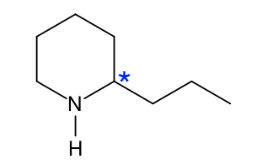
\includegraphics[width=0.8\textwidth]{coniin.png}
\end{center}
\caption{Coniin udviser stereoisomeri}
\label{fig:coniin}
\end{figure}
\noindent \textbf{b.}
Siden coniin er en middelstærk base, så gælder der
\begin{equation*}
\begin{split}
K_b = \frac{[\ce{OH-} ]^2}{c_b - [\ce{OH-}]} &\iff [\ce{OH-}]=\frac{-K_b + \sqrt{K_b^2-4 \cdot \left(-K_b \cdot c_b\right) } }{2}\\
&\iff [\ce{OH-}]=\frac{-10 ^{-pK_b} \;\unit{\textsc{m}} + \sqrt{\left(10 ^{-pK_b} \;\unit{\textsc{m}} \right) ^2-4 \cdot \left(-10 ^{-pK_b} \;\unit{\textsc{m}}\right) \cdot c_b } }{2}.
\end{split}
\end{equation*}
pH-værdien i opløsningen må da være
\begin{equation*}
\begin{split}
pH&=14,00 + \log\left(\frac{[\ce{OH-} ]}{\unit{\textsc{m}} }\right) \\
&=14,00 + \log\left(\frac{-10 ^{-pK_b} \;\unit{\textsc{m}} + \sqrt{\left(10 ^{-pK_b} \;\unit{\textsc{m}} \right) ^2-4 \cdot \left(-10 ^{-pK_b} \;\unit{\textsc{m}}\right) \cdot c_b } }{2 \;\unit{\textsc{m}} }\right) \\
&=14,00 + \log\left(\frac{-10 ^{-2,82} \;\unit{\textsc{m}} + \sqrt{\left(10 ^{-2,82} \;\unit{\textsc{m}} \right) ^2-4 \cdot \left(-10 ^{-2,82} \;\unit{\textsc{m}}\right) \cdot 0,067 \;\unit{\textsc{m}} } }{2 \;\unit{\textsc{m}} }\right) \\
&\approx 11,97.
\end{split}
\end{equation*}
I den mættede vandige opløsning af coniin har vi altså fået $pH=11,97$.\\[1ex]
\textbf{c.}
Resultaterne på de kemiske tests ses i \cref{fig:dibrom}, \cref{fig:dnph} og \cref{fig:fehling}.
\begin{multicols}{3}
\begin{figure}[H]
\begin{center}
  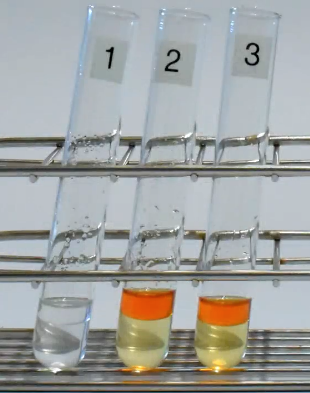
\includegraphics[width=0.333\textwidth]{dibrom.png}
\end{center}
\caption{Affarvning af bromvand}
\label{fig:dibrom}
\end{figure}
\begin{figure}[H]
\begin{center}
  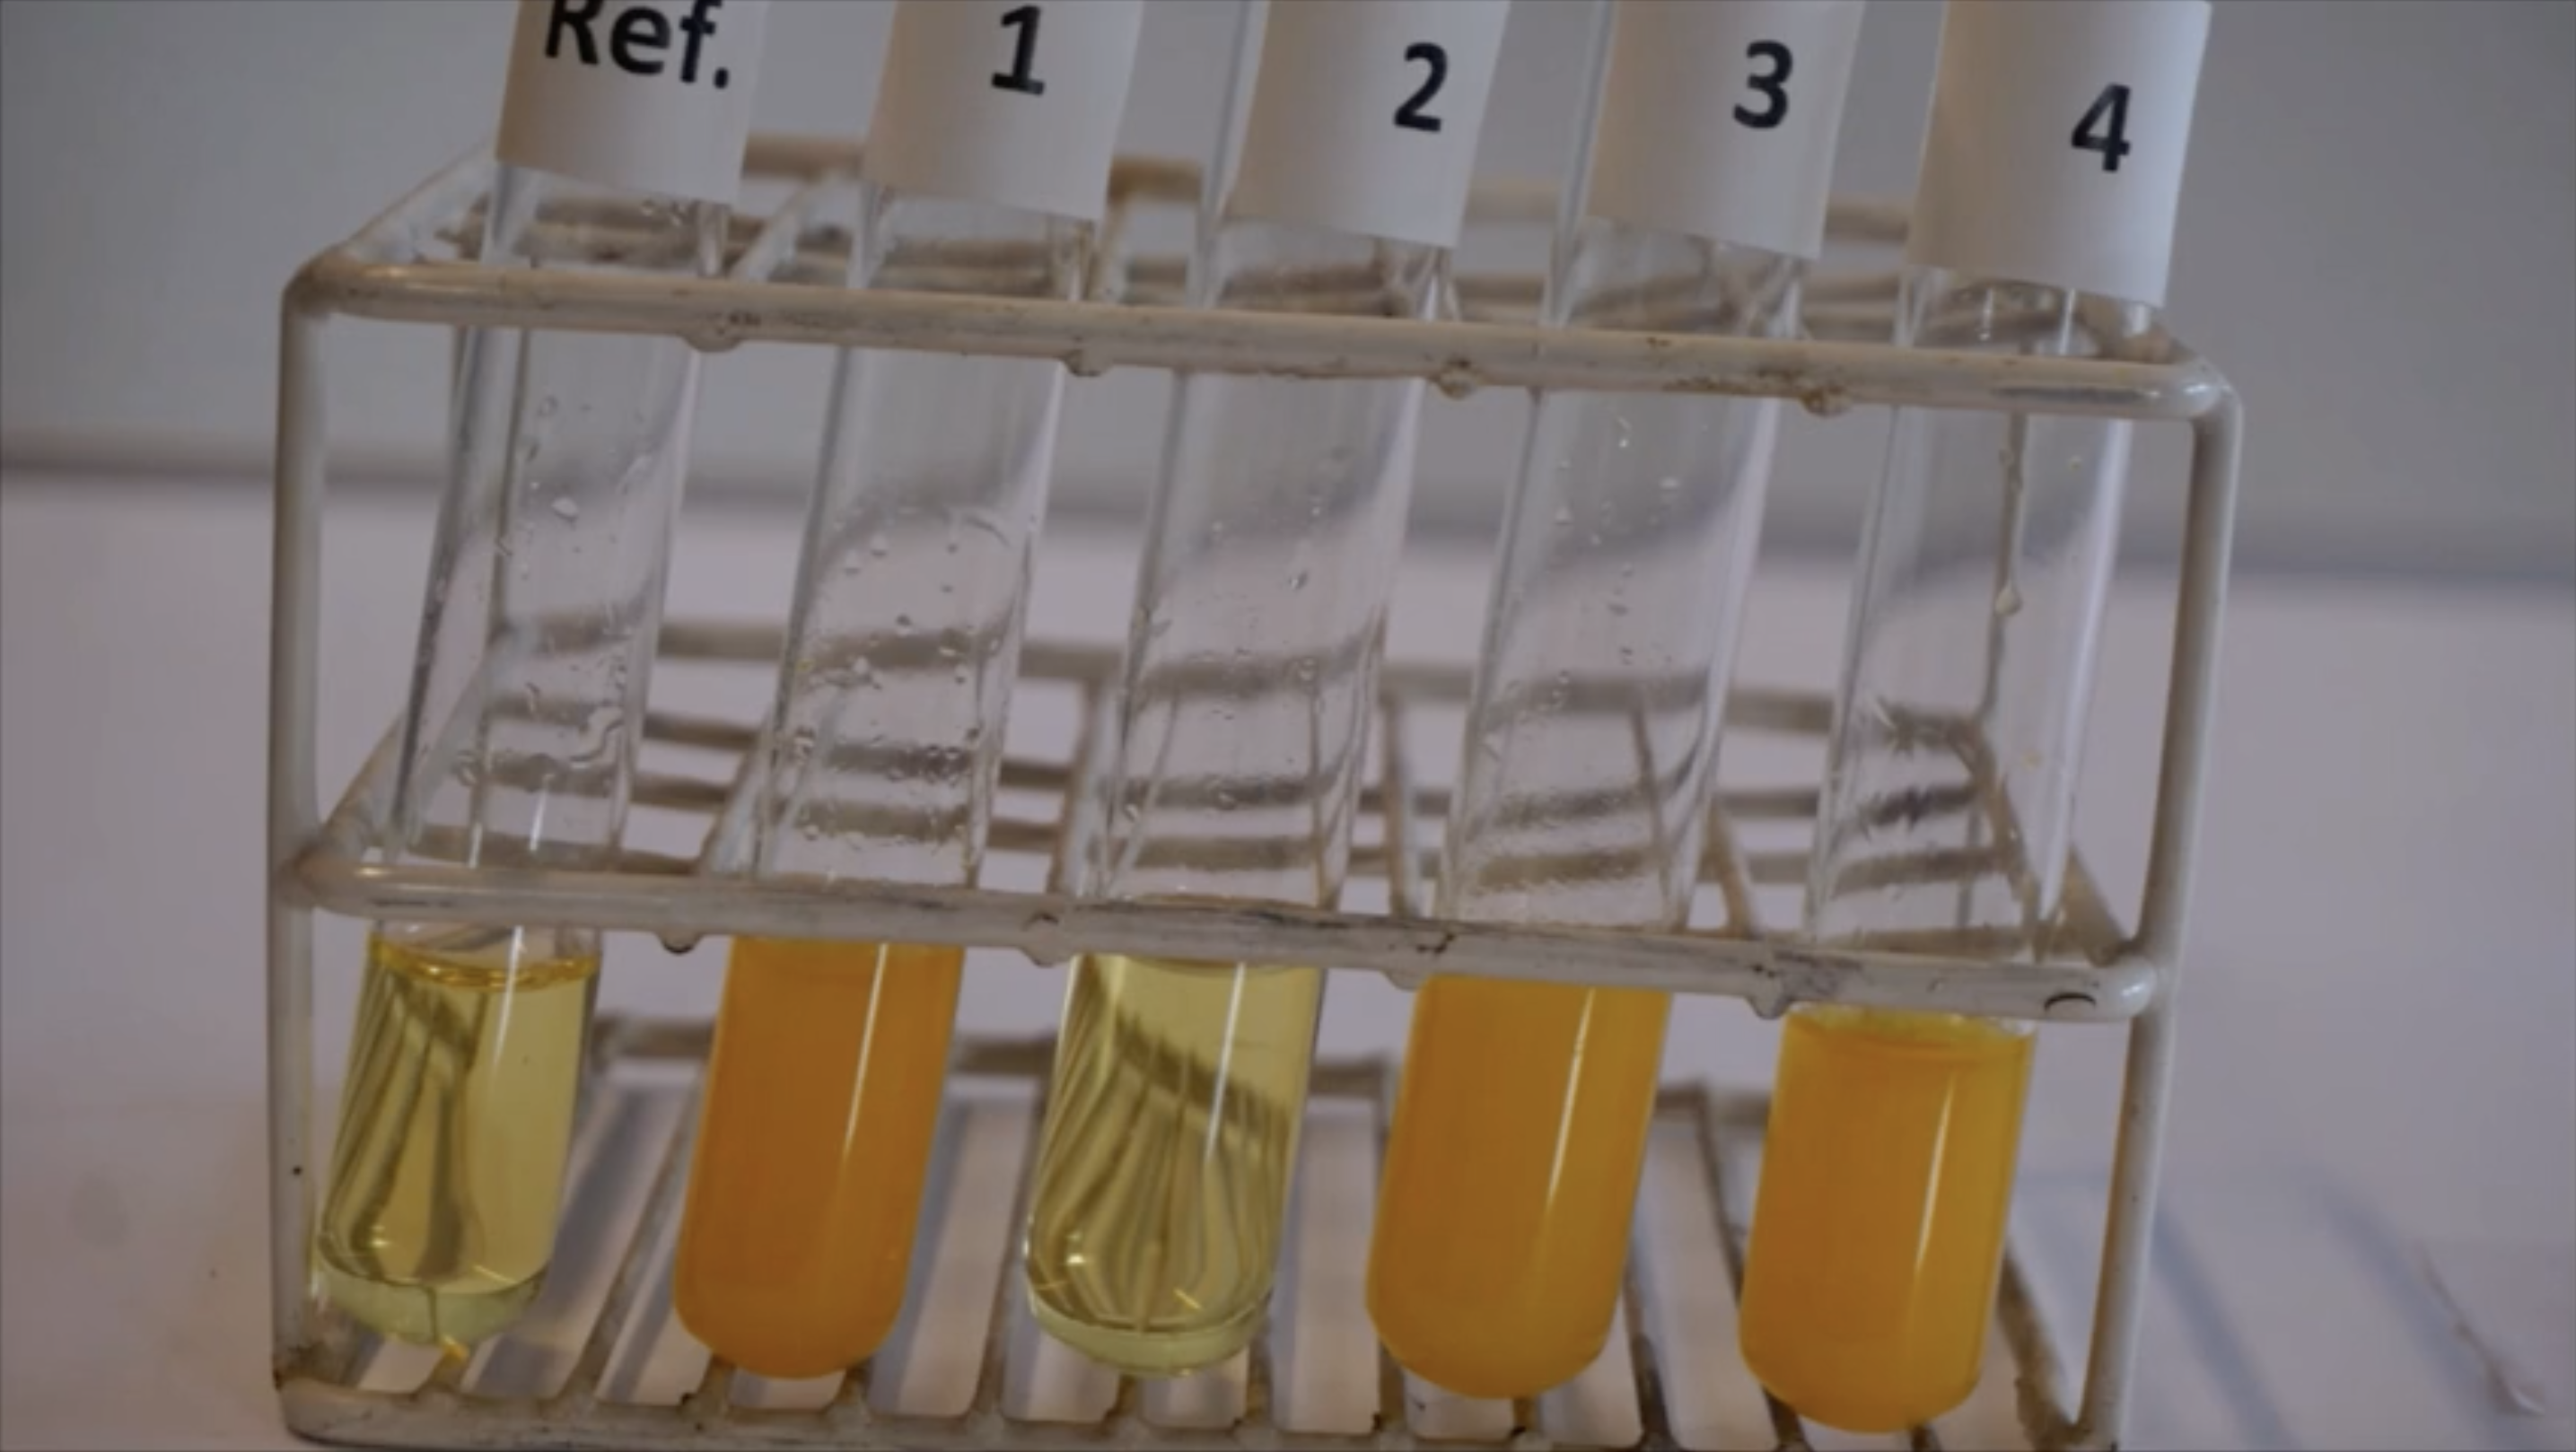
\includegraphics[width=0.333\textwidth]{dnph.png}
\end{center}
\caption{Reaktion med 2,4-dinitrophenylhydrazin}
\label{fig:dnph}
\end{figure}
\begin{figure}[H]
\begin{center}
  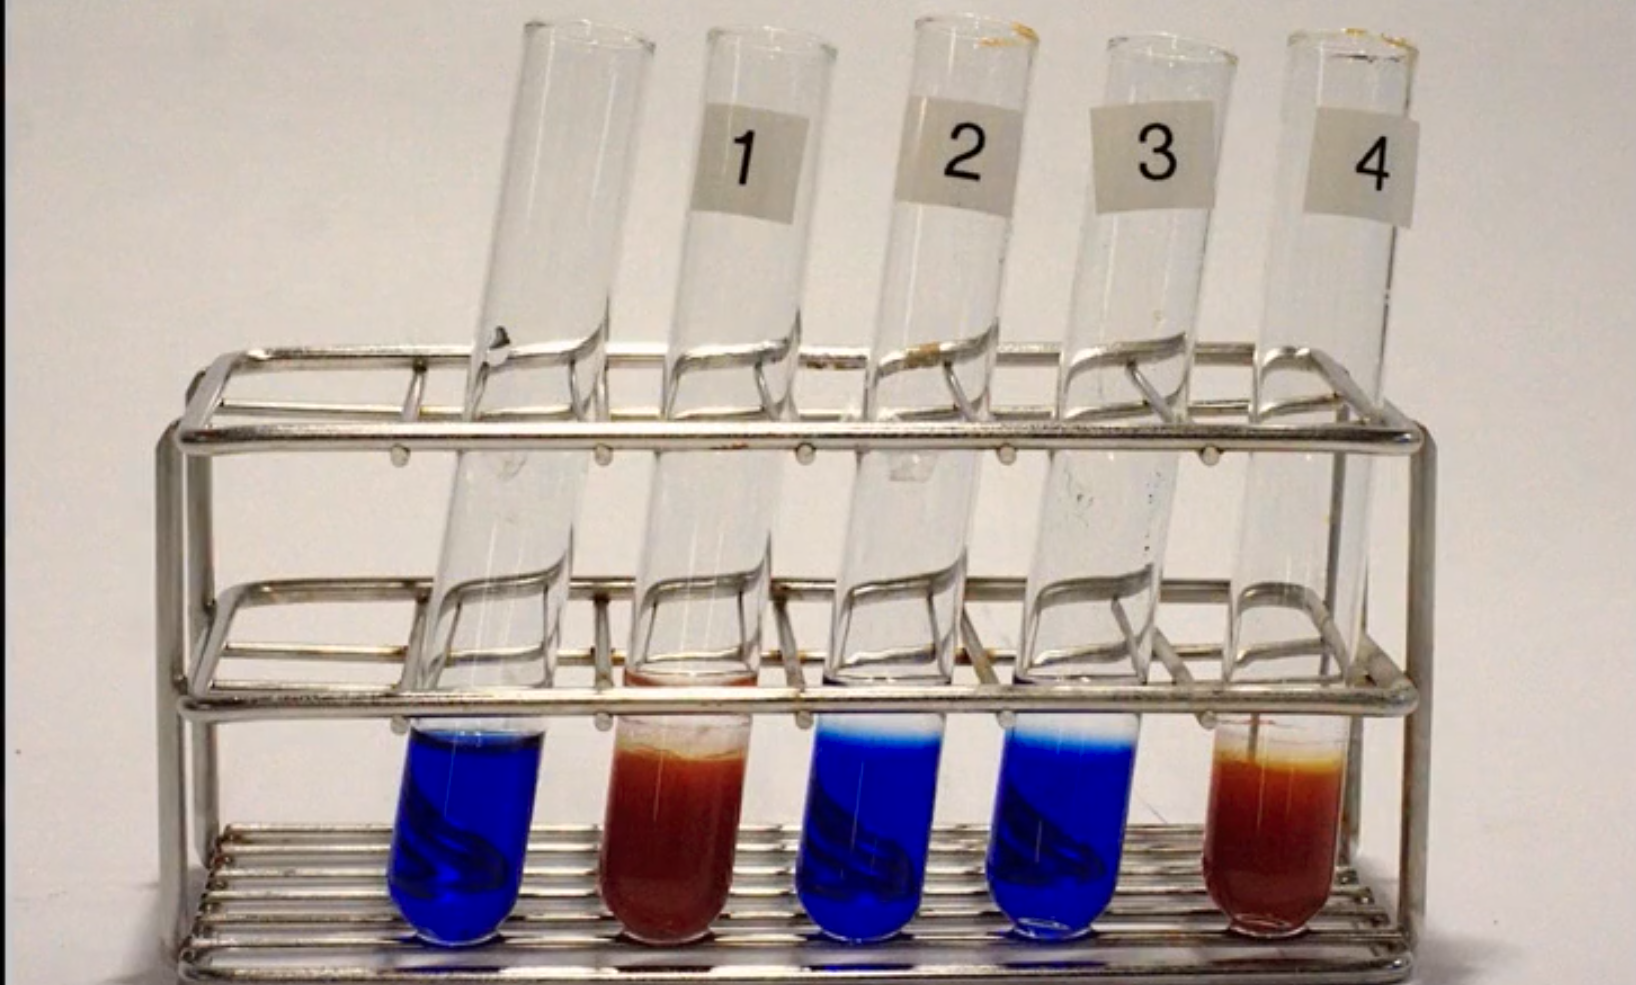
\includegraphics[width=0.333\textwidth]{fehling.png}
\end{center}
\caption{Reaktion med Fehlings væske}
\label{fig:fehling}
\end{figure}
\end{multicols}
Det ses, at stoffet i reagensglas nr. 1 adderer dibrom, men reagerer ikke med 2,4-dinitrophenylhydrazin eller Fehlings væske.
Altså må stoffet i reagensglasset indeholde en dobbeltbinding mellem to C-atomer, men er ikke en carbonylforbindelse.
Det ses i \cref{fig:ABC}, at stof B må være i reagensglas nr. 1, da det indeholder en \ce{C=C}-binding, og de to andre stoffer begge er carbonylforbindelser.

Siden stoffet i reagensglas nr. 2 reagerer med både 2,4-dinitrophenylhydrazin og Fehlings væske, så må det være en aldehyd.
Da stof A er den eneste aldehyd, så må stof A altså tilordnes reagensglas nr. 2.

Til sidst reagerer stoffet i reagensglas nr. 3 med 2,4-dinitrophenylhydrazin men ikke med Fehlings væske.
Det vil sige at stoffet i reagensglas nr. 3 må være en keton (fordi Fehlings væske som udgangspunkt kun reagerer med aldehyder, men ikke ketoner).
Siden stof C er den eneste keton, så kan reagensglas 3 altså tilordnes stof C.
\begin{figure}[H]
\begin{center}
  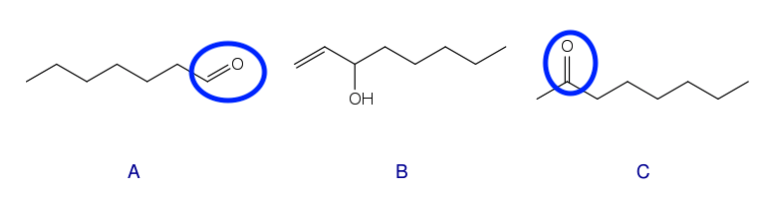
\includegraphics[width=0.8\textwidth]{ABC.png}
\end{center}
\caption{Strukturer for A, B og C}
\label{fig:ABC}
\end{figure}
\textbf{d.}
Vi starter med at se på IR-spektret for D. 
En opsummerende tabel ses i \cref{tab:IR}. 
\begin{table}[H]
\centering
\begin{tabular}{@{}llllll@{}}
\toprule
  \makecell{Bånd\\nr.} & \makecell{$\frac{1}{\lambda }$/\unit{cm^{-1}}\\(aflæst)} & Intensitet & Bindingstilordning & Kommentarer & \makecell{$\frac{1}{\lambda }$/\unit{cm^{-1}}\\(tabel)}\\
\midrule
 1 & 3000-3100 & Medium & \makecell{C-H strækning \\ C:$sp^2$} & Aromatisk ring & 3000-3100\\
  2 & 2800-2950 & Medium & \makecell{C-H strækning \\ C:$sp^3$} & \makecell{Alkyl\\ Flere bånd} & 2810-2960\\
  3 &1730 & Stærk & \ce{C=O} strækning & Ester & 1745\\
  4 & 1600 & Svag & \ce{C\bond{~-}C} strækning & Aromatisk ring & 1575-1600 \\  
  5 & 1460-1500 & Svag & \ce{C\bond{~-}C} strækning & Aromatisk ring & 1450-1500 \\  
\bottomrule
\end{tabular}
\caption{Tilordning af absorptionsbånd i IR-spektret}
\label{tab:IR}
\end{table}
Det er åbenlyst, at bånd nr. 1, 4 og 5 må komme fra den aromatiske ring.
Bånd nr. 3 skyldes \ce{C=O}-strækningsvibrationer i en estergruppe.

Vi ser nu på \ce{^1H}-NMR-spektret for X-gruppen.
En oversigt ses i \cref{tab:HNMR}.
\begin{table}[H]
\centering
\begin{tabular}{@{}lllllll@{}}
\toprule
  \makecell{Signal\\nr.} & \makecell{Kemisk skift\\(aflæst)\\$\delta$/ppm}& \makecell{Integral/areal\\(relativt antal ækvi-\\valente \ce{^1H}-atomer)}  & Opsplitning & \makecell{Antal \\nabo-\ce{^1H}'er}  & Tilordning & \makecell{Kemisk skift\\(tabel)\\$\delta$/ppm} \\
\midrule
  1 & 0,95 & 6 & Dublet & 1 & 2 \ce{C\textbf{H}3-CH} & 0,9 \\
  2 & 2,08 & 1 & Nonet & 8 & \ce{(CH3)2-C\textbf{H}-CH2-O-CO -} & 2,1\\
  3 & 4,12 & 2 & Dublet & 1 &\ce{-CH-C\textbf{H}2-O-CO-Ar} & 4,4\\
\bottomrule
\end{tabular}
\caption{Tilordning af absorptionsbånd i \ce{^1H}-NMR-spektret}
\label{tab:HNMR}
\end{table}
Signal nr. 1 kan tilordnes to ækvivalente \ce{CH3}-grupper, der kobler med \ce{^1H}-kernen hørende til en \ce{CH}-gruppe.
Det er åbenlyst, at denne \ce{CH}-gruppe kan tilordnes signal nr. 2 grundet opsplitningen.
Grundet det kemiske skift, må der indgå en estergruppe, hvilket er i overensstemmelse med IR-spektret.
Til sidst har vi fra signal nr. 3 en \ce{CH2}-gruppe, hvis \ce{^1H}-kerner kobler til \ce{^1H}-kernen hørende til signal 2.
Den eneste mulige strukturformel for X-gruppen i D ses da markeret i \cref{fig:X}.
\begin{figure}[H]
\begin{center}
  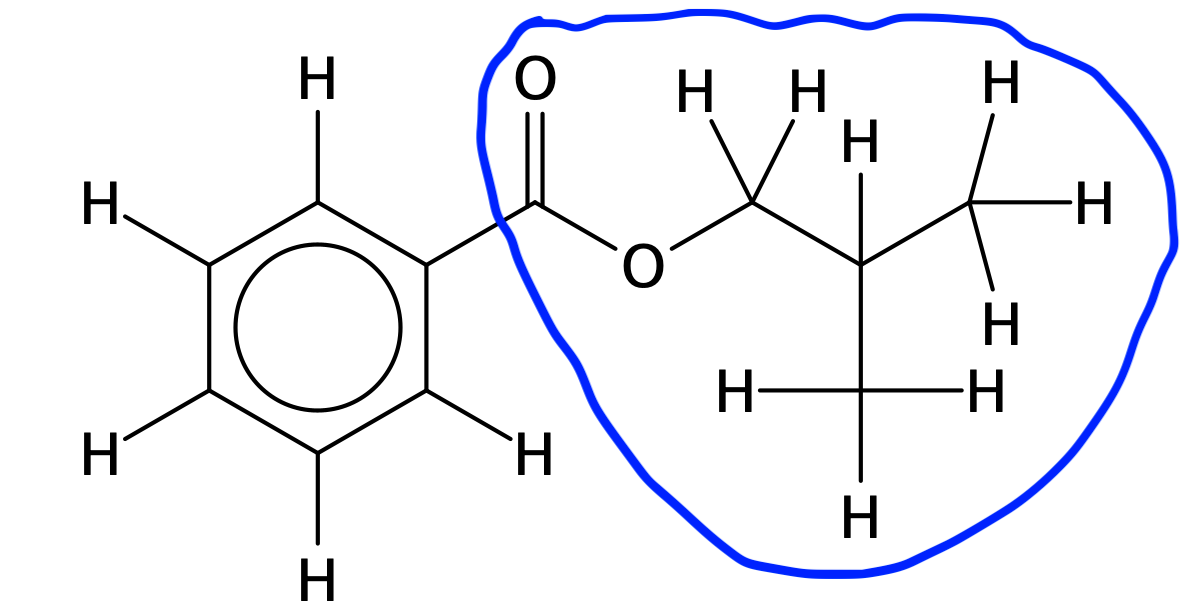
\includegraphics[width=0.8\textwidth]{X.png}
\end{center}
\caption{Strukturen for X er markeret}
\label{fig:X}
\end{figure}



\section*{Opgave 2: Brillerens}
\sol \\
\textbf{a.}
Fra videoen har vi, at der ved fremstillingen af opløsningen er benyttet 2,903 g propan-2-ol, der tilsættes vand til den har volumenet 25,0 mL.
Stofmængdekoncentrationen af propan-2-ol må da være
\begin{equation*}
\begin{split}
  c(\text{propan-2-ol} )&=\frac{n(\text{propan-2-ol} )}{V}\\
  &=\frac{m(\text{propan-2-ol} )}{M(\text{propan-2-ol}) \cdot V}\\
  &=\frac{2,903 \;\unit{g} }{60,10 \;\unit{g/mol} \cdot 25,0 \cdot 10 ^{-3} \;\unit{L} }\\
  &\approx 1,93 \;\unit{\textsc{m}}.
\end{split}
\end{equation*}
Stofmængdekoncentrationen af propan-2-ol i den fremstillede standardopløsning er altså $1,93 \;\unit{\textsc{m}} $.\\[1ex]
\textbf{b.}
Vi ser, at $c(\text{propan-2-ol} )$ er dobbelt så stor i det andet chromatogram som i det første. 
Dermed bliver volumenprocenten, og dermed arealtallet også tilnærmelsesvist dobbelt så stor.
Vi ser i \cref{fig:chroma} , at dette netop er tilfældet for den første top (ved omkring $t=100 \;\unit{s} $).
Samtidigt ser vi, at arealet under den anden top er størst i det første chromatogram og er mindre i det andet, hvilket forventes af toppen for vand (for når $c(\text{propan-2-ol} )$ forøges, så bliver volumenprocenten af vand mindre).
Det er da klart, at den første top kan tilordnes propan-2-ol, hvor den anden top kan tilordnes vand.
Dette er i overensstemmelse med, at propan-2-ol i høj grad er mindre polær end vand, og derfor hænger dårligere fast i den stationære fase, der netop er polær.
\begin{figure}[H]
\begin{center}
  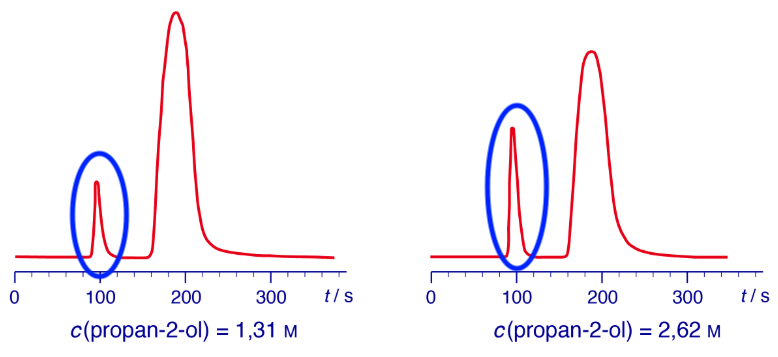
\includegraphics[width=0.8\textwidth]{chroma.png}
\end{center}
\caption{Tilordning af toppene i chromatogrammerne}
\label{fig:chroma}
\end{figure}
\noindent \textbf{c.}
Lad $A$ betegne arealtallet. 
Så har vi fra standardkurven, at
\[
A=338 \;\unit{\textsc{m} ^{-1}} \cdot c(\text{propan-2-ol} ) -4,10 \iff c(\text{propan-2-ol})=\frac{A + 4,10}{338} \;\unit{\textsc{m}}. 
\] 
Vi finder nu et udtryk for det samlede volumen af brillerens
\begin{equation*}
\begin{split}
  c(\text{propan-2-ol} )=\frac{n(\text{propan-2-ol})}{V(\text{blanding})} &\iff V(\text{blanding} )=\frac{n(\text{propan-2-ol} )}{c(\text{propan-2-ol} )}\\
  &\iff V(\text{blanding} )=\frac{338 \cdot n(\text{propan-2-ol} )}{\left(A+4,10\right) \;\unit{\textsc{m}} }.
\end{split}
\end{equation*}
Vi finder ligeledes et udtryk for volumenet af propan-2-ol i blandingen.
\begin{equation*}
\begin{split}
  \rho(\text{propan-2-ol} )=\frac{m(\text{propan-2-ol} )}{V(\text{propan-2-ol})} \iff V(\text{propan-2-ol})=\frac{m(\text{propan-2-ol})}{\rho (\text{propan-2-ol} )}.
\end{split}
\end{equation*}
Da vi kender arealtallet for propan-2-ol i Brillerens, så kan vi nu udregne volumenprocenten, som må være
\begin{equation*}
\begin{split}
  c _{\text{volumen\%} }(\text{propan-2-ol})&=\frac{V(\text{propan-2-ol} )}{V(\text{blanding} )}\\
  &=\frac{m(\text{propan-2-ol} ) \cdot (A + 4,10) \;\unit{\textsc{m}} }{n(\text{propan-2-ol} ) \cdot 338 \cdot \rho(\text{propan-2-ol} ) }\\
  &=M(\text{propan-2-ol} ) \cdot  \frac{(A + 4,10) \;\unit{\textsc{m}} }{338 \cdot \rho(\text{propan-2-ol} ) }\\
  &=60,10 \;\unit{g/mol} \cdot \frac{(988+4,10) \;\unit{\textsc{m}} }{338 \cdot 0,781 \cdot 10^3 \;\unit{g/L} }\\
  &\approx 0,226 \\
  &=22,6 \%.
\end{split}
\end{equation*}
Indholdet af propan-2-ol i Brillerens er altså $c _{\text{volumen\%} }(\text{propan-2-ol})=22,6\%$. 

\section*{Opgave 4: Nanopartikler til vandrensning}
\sol \\
\textbf{a.}
Den kemiske formel for magnesiumnitrat er \ce{Mg(NO3)2}.\\[1ex]
\textbf{b.}
Der gælder, at \ce{OH-} er en stærk base.
Fra Le Chateliers princip har vi, at et ydre indgreb vil fremkalde en forskydning, som formindsker virkningen af indgrebet.
Det er da klart, at ligevægten vil forskydes mod venstre, hvis pH sænkes.\\[1ex]
\textbf{c.}
$\Delta H \stst $ beregnes med tabelopslag, og er
\begin{equation*}
\begin{split}
  \Delta H \stst &=H \stst (\ce{MgO(s)}) + H \stst (\ce{H2O(g)})-H \stst (\ce{Mg(OH)2(s)})\\
  &=-601,60 \;\unit{kJ/mol} + (-241,8 \;\unit{kJ/mol}) -(-924,5 \;\unit{kJ/mol} )\\
  &=81,1 \;\unit{kJ/mol}.
\end{split}
\end{equation*}
Siden $\Delta H \stst >0$, så er reaktionen fra venstre mod højre endoterm.

$\Delta S \stst $ beregnes ligeledes med tabelopslag, og er
\begin{equation*}
\begin{split}
  \Delta S \stst &=S \stst (\ce{MgO(s)}) + S \stst (\ce{H2O(g)})-S \stst (\ce{Mg(OH)2(s)})\\
  &=26,95 \;\unit{\frac{J}{mol \cdot K}} + 188,8 \;\unit{\frac{J}{mol \cdot K}} -63,2 \;\unit{\frac{J}{mol \cdot K}}\\
  &=152,55 \;\unit{\frac{J}{mol \cdot K}}.
\end{split}
\end{equation*}
Siden $\Delta S \stst >0$, så øges uordenen fra venstre mod højre.
Dette er i overensstemmelse med reaktionsskemaet, hvor der er et molekyle på gasform på højre side af ligevægtspilen, men ikke venstre, og antallet af formelenheder vokser fra venstre mod højre.\\[1ex]
\textbf{d.}
Vi starter med at opskrive reaktionsbrøken, som er
\begin{equation*}
\begin{split}
  Y=p(\ce{H2O}).
\end{split}
\end{equation*}
Der gælder, at reaktionen kan forløbe spontant netop når $\Delta G <0$.
Fra sammenhængen mellem $\Delta G$ og $\Delta G \stst $ har vi så, at 
\begin{equation*}
\begin{split}
  \Delta G < 0 &\iff \Delta G \stst + R \cdot T \cdot \ln\left(Y\right) <0\\
  &\iff \Delta H \stst -T \cdot \Delta S \stst + T \cdot R \cdot \ln\left(\frac{p(\ce{H2O})}{\;\unit{bar} }\right) <0 \\
  &\iff T \cdot \left(-\Delta S \stst + R \cdot \ln\left(\frac{p(\ce{H2O} )}{\;\unit{bar} }\right) \right) < -\Delta H \stst \\
  &\iff T > \frac{\Delta H \stst }{\Delta S \stst -R \cdot \ln\left(\frac{p(\ce{H2O} )}{\;\unit{bar} }\right) },
\end{split}
\end{equation*}
hvor den sidste biimplikation gælder, da $-\Delta S \stst + R \cdot \ln\left(\frac{p(\ce{H2O} )}{\;\unit{bar} }\right)$ er en negativ størrelse. 
Vi kan nu udregne betingelsen for, at reaktionen kan forløbe spontant
\begin{equation*}
\begin{split}
  T &> \frac{\Delta H \stst }{\Delta S \stst -R \cdot \ln\left(\frac{p(\ce{H2O} )}{\;\unit{bar} }\right) }\\
  &=\frac{81,1 \cdot 10^3 \;\unit{J/mol} }{152,55 \;\unit{\frac{J}{mol \cdot K}} -8,314 \;\unit{\frac{J}{mol \cdot K}} \cdot \ln\left(\frac{0,030 \;\unit{bar} }{\;\unit{bar} }\right) }\\
  &\approx 446 \;\unit{K}.
\end{split}
\end{equation*}
Temperaturen skal altså være større end $446 \;\unit{K} $ for at reaktionen kan forløbe spontant, når partialtrykket af vand er $0,030 \;\unit{bar} $. 



\end{document}
